\chapter{Discussion}\label{chapter:discussion}

This master thesis investigated whether GraphQL can bring performance improvement in micro-frontend architectures. The results of the evaluation of the prototype implementation of the micro-frontend architecture are discussed in this chapter. The results from Chapter \ref{chapter:results} are used to make a statement about the hypothesis from Chapter \ref{chapter:introduction}.


\section{Request Size}

Figure \ref{fig:discussion:request-size} displays the results already shown in the previous chapter as a bar chart. In terms of request size, the three approaches are not very far apart from each other. The reduction of queries only makes 1.64 KB difference, in contrast to only sharing the cache.

\begin{figure}[H]
  \centering
  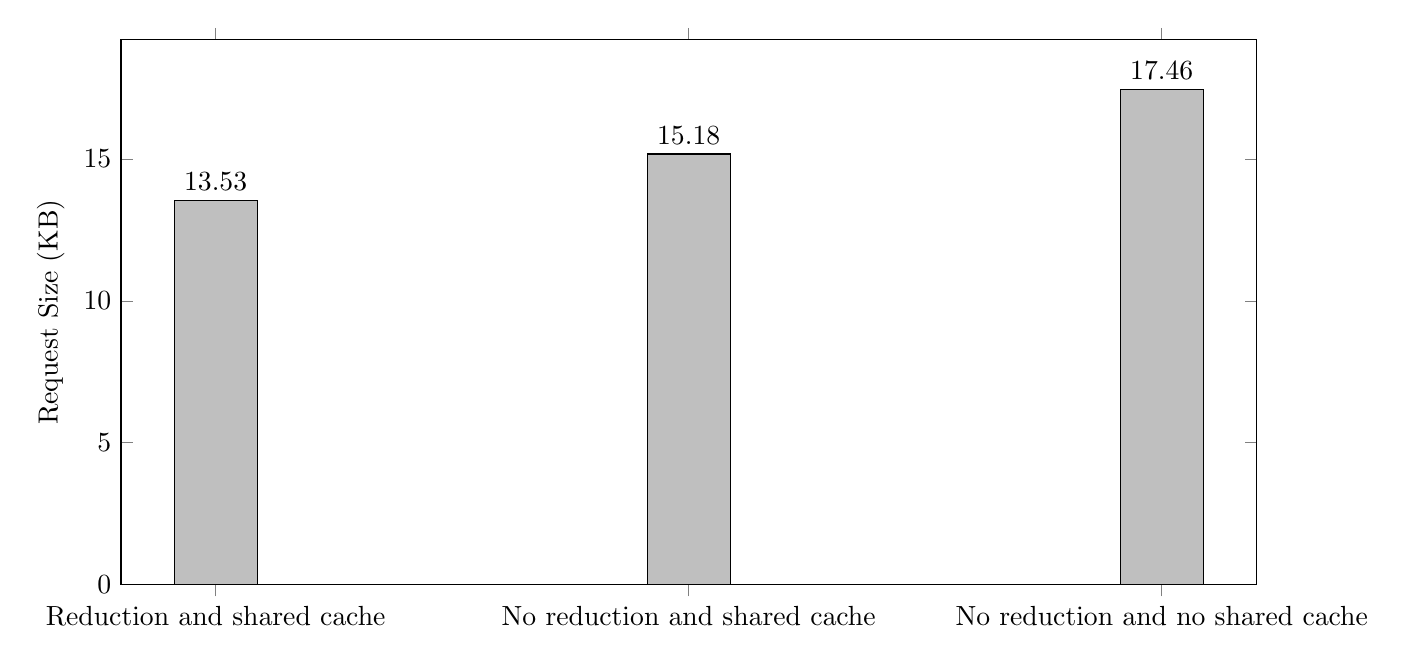
\begin{tikzpicture}
    \begin{axis}[
      ymin=0,
      ybar,
      ylabel={Request Size (KB)},
      xtick=data, 
      symbolic x coords={Reduction and shared cache, No reduction and shared cache, No reduction and no shared cache}, 
      nodes near coords align={vertical},
      nodes near coords,
      height=8.5cm,
      width=16cm,
      bar width=30pt,
      cycle list={
        {fill=lightgray, draw=gray}
      },
    ]
    \addplot coordinates {(Reduction and shared cache, 13.53) (No reduction and shared cache, 15.18) (No reduction and no shared cache, 17.46)};
    \end{axis}
  \end{tikzpicture}
  \caption{Request size comparison of the three approaches.}\label{fig:discussion:request-size}
\end{figure}

\section{Response Size}

Figure \ref{fig:discussion:response-size} displays the results already shown in the previous chapter as a bar chart. In contrast to the request size, the response sizes are very far apart. When comparing the naive approach with the two improved approaches, there is a difference of about 2.40 MB. However, when comparing the two improved approaches, the difference is not very large. For the records that the application fetches, the reduction does not make such a big difference, in terms of responses.

\begin{figure}[H]
  \centering
  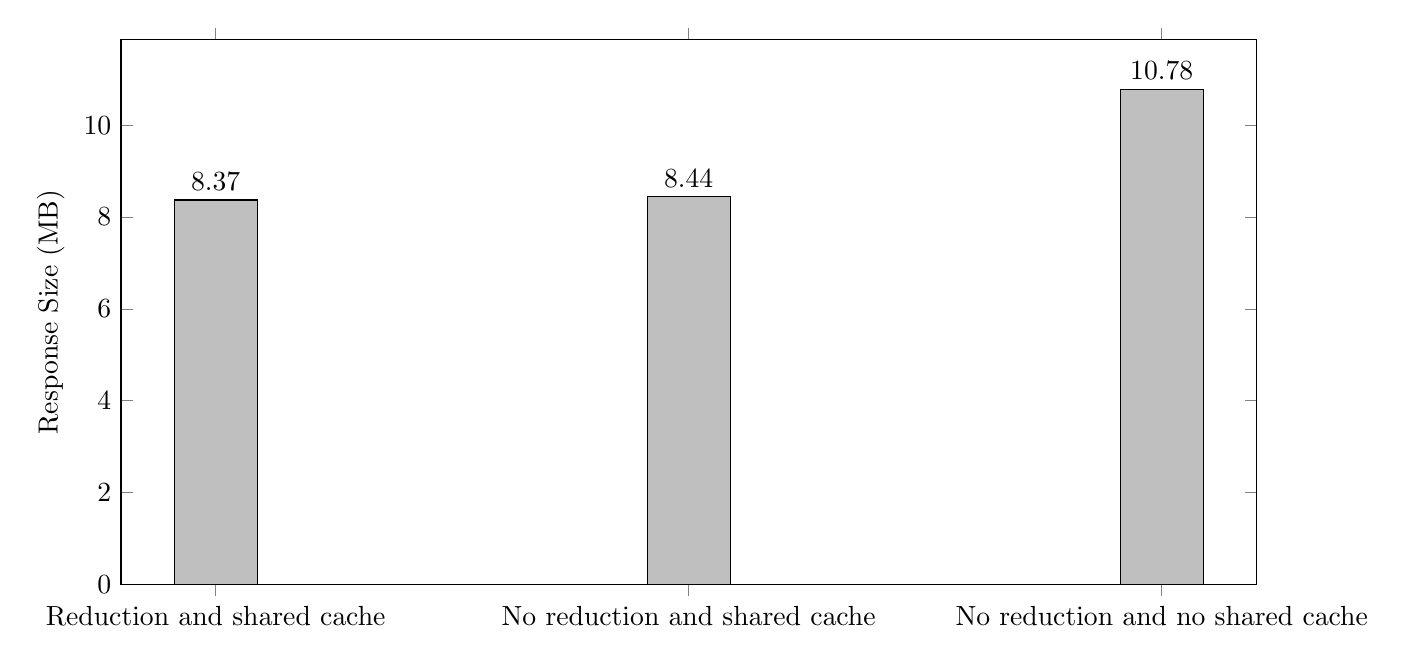
\begin{tikzpicture}
    \begin{axis}[
      ymin=0,
      ybar,
      ylabel={Response Size (MB)},
      xtick=data, 
      symbolic x coords={Reduction and shared cache, No reduction and shared cache, No reduction and no shared cache}, 
      nodes near coords align={vertical},
      nodes near coords,
      height=8.5cm,
      width=16cm,
      bar width=30pt,
      cycle list={
        {fill=lightgray, draw=gray}
      },
    ]
    \addplot coordinates {(Reduction and shared cache, 8.37) (No reduction and shared cache, 8.44) (No reduction and no shared cache, 10.78)};
    \end{axis}
  \end{tikzpicture}
  \caption{Response size comparison of the three approaches.}\label{fig:discussion:response-size}
\end{figure}
